\documentclass[11pt]{article}
\usepackage[utf8]{inputenc}
\usepackage{centernot}
\usepackage[parfill]{parskip}
\usepackage{amsmath}
\usepackage{amssymb}
\usepackage{graphicx}
\begin{document}
\title{Analys Problem 3}
\author{Robin Boregrim}
\maketitle
\renewcommand{\contentsname}{Innehållsförteckning}
\tableofcontents
\newpage
\section{Uppgiften}
Undersök funktionen
$$f(x) = e^{-x} -e^{-2x}$$
med avseende på extrempunkter, asymptoter och konvexitetsegenskaper. Skissa även grafen.
\section{Lösning}
\subsection{Nollställen}
Vi börjar med att beräkna nollställen för funktionen $f(x)$.
$$f(x) = e^{-x} -e^{-2x} = 0$$
$$e^{-x} = e^{-2x}$$
Vi tar $\ln$ av båda led.
$$\ln(e^{-x}) = \ln(e^{-2x})$$
$$-x\ln(e) = -2x\ln(e)$$
$$-x = -2x$$
och adderar $ + 2x$ i båda led,
$$x = 0.$$
Då vet vi att $f(x)$ har nollstället $$f(0) = 0.$$
\subsection{Extrempunkter}
För att beräkna extrempunkter så behöver vi beräkna nollställen för $f'(x)$, derivatan av $f(x)$.
$$f'(x) = 2e^{-2x} -e^{-x}.$$
Vi sätter $f'(x) = 0$ och förenklar.
$$f'(x) = 2e^{-2x} -e^{-x} = 0$$
$$2e^{-2x} = e^{-x}$$
$$\ln(2e^{-2x}) = \ln(e^{-x})$$
$$\ln2 + \ln(e^{-2x}) = \ln(e^{-x})$$
$$\ln2 -2x \ln(e) = -x\ln(e)$$
$$\ln2 -2x= -x$$
Vi adderar $ + 2x$ i båda led.
$$\ln2 = x$$\\
Nu när vi vet att $f'(\ln2) = 0$ så kan vi beräkna om $f(\ln2)$ är en maxi-, mini- eller terrasspunkt. Detta gör vi genom att kolla om $f'(x)$ är positiv eller negativ för $x$ större och mindre än $\ln2$.
Eftersom $x = \ln2$ är den enda nollpunkten för $f'$ så behöver vi bara beräkna ett värde över och ett värde under $x=\ln2$.\\
För $x < \ln2$:
$$\frac{1}{2}< \ln2$$
$$f'(\frac{1}{2}) = 2e^{-\frac{2}{2}} -e^{-\frac{1}{2}}$$
$$= \frac{2}{e} - \frac{1}{\sqrt{e}}$$
$$= \frac{2}{e} - \frac{\sqrt{e}}{e}$$
$$=\frac{2- \sqrt{e}}{e}$$
Eftersom $$2 > \sqrt{e}$$ så är
$$\frac{2- \sqrt{e}}{e} = f'(\frac{1}{2}) > 0$$\\
För $x > \ln2$:
$$1 > \ln2$$
$$f'(1) = 2e^{-2} -e^{-1}$$
$$= \frac{2}{e^2} - \frac{1}{e}$$
$$= \frac{2-e}{e^2}$$
Eftersom $$2 < e$$ så är
$$\frac{2-e}{e^2} = f'(1) < 0$$\\
För skissen kan det även vara bra att veta vad $f(\ln2)$ är, så vi beräknar det.
$$f(\ln2) = e^{-\ln2} -e^{-2\ln2} = \frac{1}{2} -\frac{1}{4} = \frac{1}{4}$$
Nu kan vi sammanställa detta i en tabell.
$$
\begin{tabular}{c|c|c|c}
x&&$\ln2$&\\ \hline
f'&+&0&- \\
f& $\nearrow$ & $\frac{1}{4}$&$\searrow$
\end{tabular}$$

\subsection{Konvexitet}
För att beräkna konvexitet kan vi använda $f''(x)$, andraderivatan till $f(x)$.
$$f''(x) = e^{-x} -4e^{-2x}$$
Först, precis som med $f'(x)$, så försöker vi hitta nollpunkter.
$$f''(x) = e^{-x} -4e^{-2x} = 0$$
$$e^{-x} = 4e^{-2x}$$
$$\ln(e^{-x}) = \ln(4e^{-2x})$$
$$\ln(e^{-x}) = \ln4 + \ln(e^{-2x})$$
$$-x\ln(e) = \ln4 + -2x\ln(e)$$
$$-x = \ln4 -2x$$
$$x = \ln4$$

Nu när vi vet nollpunkten för $f''(x)$ kan vi beräkna om $f''(x)$ är posetiv eller negativ för $x$ större eller mindre än $\ln4$.\\
För $x < \ln4$:
$$e^{-1} -4e^{-2}$$
$$=\frac{1}{e} -\frac{4}{e^{2}}$$
$$=\frac{e-4}{e^{2}}$$
Eftersom $$e<4$$
så är $$ \frac{e-4}{e^{2}} = f''(x) < 0$$
Vilket betyder att $f(x)$ är konkav för $x < \ln4$.


För $x > \ln4$:
$$e^{-2} -4e^{-2\cdot 2}$$
$$=\frac{1}{e^{2}} -\frac{4}{e^{4}}$$
$$=\frac{e^2 - 4}{e^{4}}$$
Eftersom $$e^2 > 4$$
så är $$ \frac{e-4}{e^{2}} = f''(x) > 0$$
Vilket betyder att $f(x)$ är konvex för $x > \ln4$.

Precis som med första derivatan så vill vi för referens för skissen även veta vad $f(\ln4)$ är.
$$f(\ln4) = e^{-\ln4} -e^{-2\ln4}$$
$$= \frac{1}{4} - \frac{1}{4^2}$$
$$= \frac{4}{16} - \frac{1}{16}$$
$$= \frac{4}{16} - \frac{1}{16}$$
$$= \frac{3}{16}$$
Nu kan vi sammanställa detta i en tabell.
$$
\begin{tabular}{c|c|c|c}
x&&$\ln4$&\\ \hline
f'&-&0&+ \\
f& $\frown$ & $\frac{3}{16}$&$\smile$
\end{tabular}$$
\subsection{Asymptoter}
För att beräkna asymptoter så använder vi oss av att asymptoten $kx+m$ för $f(x)$ när $x$ går mot $a$ är  
$$ \lim_{x\to a} \frac{f(x)}{x} = k$$
$$ \lim_{x\to a} f(x)-kx = m$$
Eftersom $f(x)$ är kontinuerlig så finns det bara två möjliga asymptoter som är $x\to\infty$ eller $x\to-\infty$.\\

$x\to\infty$:
$$k = \lim_{x\to\infty}(\frac{e^{-x} -e^{-2x}}{x}) = \lim_{x\to\infty}((\frac{1}{e^x} - \frac{1}{e^{2x}})  \cdot \frac{1}{x}) = (0 - 0) \cdot 0 = 0$$
$$m = \lim_{x\to\infty} (e^{-x} -e^{-2x} - 0x ) = \lim_{x\to\infty}(\frac{1}{e^x} - \frac{1}{e^{2x}}) = 0-0 = 0$$
Detta betyder att det finns en vågrät asymptot där $y=0$ för $x\to\infty$.\\

$x\to-\infty$:
$$k = \lim_{x\to -\infty}(\frac{e^{-x} -e^{-2x}}{x}) = \lim_{x\to -\infty}((1- e^{-x}) \cdot \frac{e^{-x}}{x}) = \lim_{x\to \infty}((e^{x}-1) \cdot \frac{e^{x}}{x}) = \infty.$$
Detta betyder att det inte finns någon asymptot för $x\to-\infty$.
\newpage
\subsection{Skiss}
För att skissa grafen så sätter vi först ut viktiga punkter som vi vet att grafen går igenom, dvs nollstället, extrempunkten $\frac{1}{4}$ och där grafen går från konkav till konvex $\frac{3}{16}$.\\

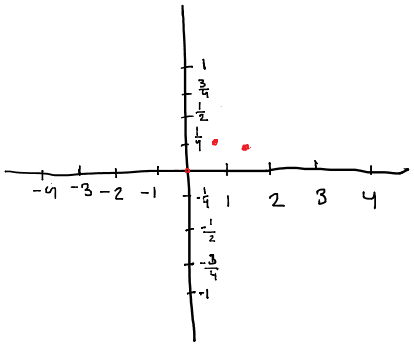
\includegraphics[height=5cm]{skiss1}\\
Sen använder vi oss av dessa punkter, vad vi vet från grafens konvexitet och asymptoten ($y=0, x\to\infty$) för att rita ut grafen $f(x)$. \\
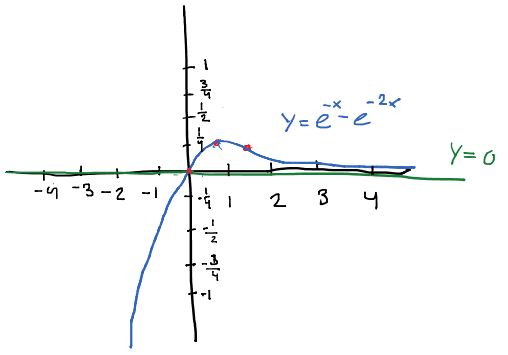
\includegraphics[height=5cm]{skiss2}
\end{document}